% !TEX encoding = UTF-8
% !TEX TS-program = pdflatex
% !TEX root = ../relazione-finale.tex

%**************************************************************
\pagebreak
\chapter{Svolgimento dello stage}
\label{cap:descrizione-stage}
%**************************************************************

\intro{Nelle sezioni di questo capitolo parlerò dell'effettivo svolgimento dello stage: organizzazione dello
stage, analisi dei requisiti, progettazione ad alto livello, documentazione prodotta, test sviluppati e
validazione dei requisiti.}\\

%**************************************************************
\section{Organizzazione dello Stage}

La pianificazione, in termini di quantità di ore di lavoro, è stata distribuita secondo la tabella ~\ref{tab:organizzazione-stage}:

\begin{tabular}{|>{\centering} m{1.5cm}|>{\centering} m{1.5cm}|m{10cm}|}
	\hline
	\multicolumn{2}{|c|}{\textbf{Durata in ore}} & \textbf{Descrizione dell'attività} \\
	\hline
	\multicolumn{2}{|c|}{40} & Formazione
	 \begin{itemize}
		\item Architettura microservizi
		\item Node.JS orientato ai microservizi
		\item React
	\end{itemize} 
	\\
	\hline
	
	\multirow{4}{*}{120} & & Analisi, sviluppo e implementazione servizio di comunicazione con i dispositivi IoT\\
	\cline{2-2}
	& 40 & \begin{itemize}
		\item Analisi dei protocolli open source esistenti per i diversi dispositivi IoT
		\item Stima implementazione eventuali nuovi protocolli
	\end{itemize} \\
	\cline{2-2}
	& 80 & \begin{itemize}
		\item Progettazione del servizio di comunicazione con i dispositivi
		\item Progettazione dei test del servizio di comunicazione
		\item Realizzazione dei test e del servizio di comunicazione in Node.js
	\end{itemize} \\
	\hline
	
	\multirow{4}{*}{120} & & Analisi, sviluppo e implementazione servizio di presentazione delle informazioni agli utenti\\
	\cline{2-2}
	& 40 & \begin{itemize}
		\item Analisi interazione utente con la \textit{dashboard}
	\end{itemize} \\
	\cline{2-2}
	& 80 & \begin{itemize}
		\item Progettazione del servizio di presentazione informazioni
		\item Progettazione dei test del servizio di presentazione
		\item Realizzazione dei test e del servizio di presentazione in React, HTML5 e CSS3.
	\end{itemize} \\
	\hline
	
	\multicolumn{2}{|c|}{20} & {\textit{Review} dei servizi, \textit{deploy} dei servizi su Heroku.}\\
	\hline
	
	\multicolumn{2}{|c|}{\textbf{Totale ore}} & {\textbf{300}} \\
	\hline
	
\end{tabular}
% Le settimane sono composte da 40 ore totali di impegno sul progetto, 

\clearpage
\section*{Milestone}
In questa sezione vengono presentate le milestone previste per il progetto su base settimanale, associando a ciascuna milestone i prodotti che devono essere sviluppati entro la corrispondente scadenza.
\begin{itemize}
	\item Prima settimana: Completamento delle attività di autoformazione con produzione di una breve relazione riguardante la stessa;
	\item Seconda e terza settimana: Analisi dei protocolli di comunicazione esistenti, primo ciclo di progettazione e implementazione del servizio di comunicazione, mirato all'implementazione dei dispositivi \textit{virtualizzati};
	\item Quarta e quinta settimana: Revisione analisi sui protocolli, secondo ciclo di progettazione e implementazione del servizio di comunicazione, mirato all'implementazione dei dispositivi fisici (Raspberry Pi);
	\item Sesta e settima settimana: Analisi dell'interazione utente con la dashboard, progettazione e implementazione del servizio di presentazione;
	\item Ottava settimana: Revisione dei servizi, stesura del Manuale d'Uso e deploy (opzionale) di un ambiente di simulazione della dashboard su Heroku.
\end{itemize}

%**************************************************************
\section{Ambiente di sviluppo}

Sistemi operativi, dispositivi e tecnologie utilizzate.

In questa sezione sono descritte le tecnologie e gli strumenti di sviluppo che ho utilizzato per lo sviluppo del progetto, includendo la motivazione per cui ho fatto la scelta.
Nella tabella ~\ref{tab:tecnologie} è presente un sommario delle tecnologie di cui approfondisco nelle sotto-sezioni seguenti. Allo stesso modo, la tabella ~\ref{tab:strumenti} include il sommario degli strumenti che ho utilizzato per lo sviluppo del prototipo. 

\begin{table}[H]
\caption{Tabella con il sommario delle tecnologie utilizzate}
\label{tab:tecnologie}
\begin{tabularx}{\linewidth}{|c|X|}
\hline
\textbf{Tecnologia} & \textbf{Descrizione}\\
\hline
Node.js & Node.js è un'ambiente d'esecuzione utilizzato per l'implementazione di applicazioni server in JavaScript. \\
\hline
React & React è una libreria per il linguaggio JavaScript il cui scopo è costruire interfacce utente. \\
\hline
EcmaScript 2017 & EcmaScript è un linguaggio di programmazione la cui implementazione standard più conosciuta è JavaScript. \\
\hline
Jest & Jest è un \emph{framework} per l'implementazione di test per codice JavaScript. \\
\hline
ESLint & ESLint è uno strumento \emph{open source} per l'analisi statica del codice JavaScript prodotto. \\
\hline
HTML5 & HTML5 è un linguaggio di markup per la formattazione e impaginazione delle pagine Web pubblicato come W3C Recommendation dall'ottobre 2014. \\
\hline
CSS3 & CSS3 è un linguaggio di formattazione delle pagine Web. \\
\hline
Docker & Docker è una .... \\
\hline
\end{tabularx}
\end{table}

\begin{table}[H]
\caption{Tabella con il sommario degli strumenti di sviluppo utilizzati}
\label{tab:strumenti}
\begin{tabularx}{\linewidth}{|c|X|}
\hline
\textbf{Strumento} & \textbf{Descrizione}\\
\hline
Atom & Atom è un editor di testo sviluppato da GitHub con tecnologie moderne e personalizzabile. \\
\hline
Visual Studio Code & Visual Studio Code è un editor di testo sviluppato da Microsoft specificatamente per i linguaggi del Web. \\
\hline
Jest (CLI) & Jest (CLI) è l'interfaccia a linea di comando per l'esecuzione dei test sviluppati con il framework Jest. \\
\hline
Docker (engine) & L'engine Docker è una .... \\
\hline
Docker (compose) & Docker compose è ... \\
\hline
\end{tabularx}
\end{table}

\subsection{Node.js}

Node.js è un'ambiente d'esecuzione multipiattaforma open source per JavaScript e utilizzato per l'implementazione di applicazioni server in JavaScript.

Per consentire l'esecuzione di JavaScript lato server, Node.js utilizza il motore di esecuzione JavaScript **V8** sviluppato da Google per il browser Chrome.

Ho riassunto gli aspetti positivi della piattaforma Node.js nei seguenti punti: 
\begin{itemize}
  \item Node.js utilizza il modello \emph{event-driven} per la gestione delle operazioni di \emph{input} e \emph{output} (I/O) e in questo modo semplifica la gestione asincrona delle richieste concorrenti.
  \item Node.js utilizza JavaScript, un linguaggio di programmazione dalla sintassi semplice da imparare.
  \item Node.js utilizza npm per la gestione delle librerie dell'applicazione. Npm è il più grande registro di componenti di codice riusabile \footcite{}.
\end{itemize}

Come tutte le tecnologie, anche Node.js ha i suoi aspetti negativi, che presento di seguito:
\begin{itemize}
  \item Node.js non sfrutta i molti core presenti nelle CPU moderne e quindi operazioni fortemente CPU-bound congelano l'intero ciclo di eventi fino al termine dell'esecuzione dell'operazione.
  \item Node.js favorisce l'utilizzo del Design Pattern \emph{callback}, tuttavia in funzioni complesse si potrebbe incorrere in una eccessiva complessità nella lettura del codice.
\end{itemize}

\subsection{React}

React è una libreria per il linguaggio JavaScript il cui scopo è costruire interfacce utente.

Ho riassunto gli aspetti positivi della libreria React nei seguenti punti:
\begin{itemize}
	\item React utilizza un DOM virtuale per disegnare le interfacce, raggiungendo performance ed efficienza elevate. Grazie alla sua struttura a componenti, un aggiornamento ad uno di essi non richiede l'aggiornamento degli altri.
	\item I componenti sviluppati possono essere riutilizzati, garantendo un aumento di produttività degli sviluppatori.
	\item I dati in React seguono un flusso unidirezionale, in cui i componenti figli non possono modificare dati dei loro genitori, semplificando la manutenzione dei componenti.
\end{itemize}

Il difetto principale che attribuisco a React consiste nella sua elevata dinamicità: dal momento che gli sviluppatori di React aggiornano repentinamente le versioni rilasciate (la versione utilizzata durante lo stage è la "16.2.0"), gli sviluppatori devono mantenere aggiornati i \emph{codebase} per tutte le nuove funzionalità inserite.

\subsection{ECMAScript 2017}

ECMAScript 2017 è un linguaggio di programmazione standardizzato la cui ratifica è avvenuta nel giugno del 2017. L'implementazione dello standard più conosciuta è JavaScript.

L'edizione 2017 dello standard porta in dote le seguenti funzionalità:
\begin{itemize}
	\item Nuova sintassi per le **funzioni asincrone**. La keyword `async` indica che una funzione o un metodo ritornano una Promise, ossia una classe di oggetti che evidenziano l'asincronia dell'operazione da eseguire. La keyword `await` aspetta che la funzione asincrona termini la sua esecuzione, ritornando il risultato della Promise.
	\item Supporto iniziale per l'elaborazione multithread, attraverso tipi di oggetti immutabili e condivisibili tra thread.
	\item Nuovi metodi per gli oggetti esistenti nel linguaggio (enumerazione dei membri di un oggetto e ulteriori funzionalità di manipolazione di stringhe).
\end{itemize}

Nella mia analisi ho riscontrato che gli aspetti positivi consistono nei seguenti punti:
\begin{itemize}
	\item La nuova sintassi per la scrittura di funzioni asincrone è molto facilmente leggibile in quanto ricorda una programmazione sequenziale.
	\item Il supporto per l'elaborazione multithread consente a chi ha necessità e competenza di poter sfruttare le architetture a molti core delle moderne CPU, favorendo l'utilizzo di JavaScript anche per la programmazione di codice parallelo per le GPU.
	\item Poche nuove funzionalità rispetto alle edizioni precedenti permettono di imparare le nuove con maggior semplicità.
\end{itemize}

mentre gli aspetti negativi:
\begin{itemize}
	\item Con la nuova sintassi per le funzioni asincrone è molto facile dimenticarsi della natura asincrona del codice scritto, omettendo quindi la keyword `await`.
	\item Il supporto alla nuova edizione dello standard è presente in maniera completa solamente nelle ultime versioni dei browser e di Node.js.\footnote{\begin{itemize}
		\item Tabella di compatiblità dei browser: \href{http://kangax.github.io/compat-table/es2016plus/}{http://kangax.github.io/compat-table/es2016plus/} 
		\item Tabella di compatiblità di Node.js: \href{http://node.green/#ES2017}{http://node.green/#ES2017}
	\end{itemize}}
\end{itemize}

\subsection{Jest}

Jest è un framework per l'implementazione di test per codice scritto in JavaScript sviluppato da Facebook.

Tra gli aspetti positivi, ho riscontrato che:
\begin{itemize}
	\item Jest non richiede una configurazione, utilizzando impostazioni predefinite ottimali.
	\item Jest è una piattaforma di test completa che include strumenti di validazione dei risultati e  strumenti per il mocking.
	\item Jest comprende funzionalità per i test di regressione dei componenti scritti in React.
	\item Jest per default esegue i test parallelamente, velocizzando i processi di test.
\end{itemize}

Il difetto più grave che attribuisco a Jest consiste nella sua minor flessibilità rispetto ad altre librerie di test, quali ad esempio Mocha.

\subsection{ESLint}

ESLint è uno strumento che esegue analisi del codice sorgente scritto in JavaScript alla ricerca di bug noti, di inconsistenze di stile nella scrittura del codice e mira a mantenere il codice facilmente leggibile e manutenibile.

Gli aspetti positivi di ESLint che ho riscontrato sono:
\begin{itemize}
	\item ESLint è altamente configurabile, permettendo la definizione di regole condivise più appropriate per il proprio progetto.
	\item É supportato da molti strumenti di sviluppo.
	\item Le regole di analisi sono ben documentate, con esempi sul loro utilizzo, e gli errori emessi sono facilmente comprensibili.
\end{itemize}

L'aspetto negativo principale riscontrato ad ESLint risiede nella sua curva di apprendimento per l'installazione e l'utilizzo: ESLint infatti richiede una configurazione iniziale non banale per il suo utilizzo.

\subsection{HTML5 & CSS3}

HTML5 e CSS3 sono le ultime revisioni stabili rispettivamente del linguaggio HTML e del linguaggio CSS rilasciate dalla W3C.

Gli aspetti positivi di queste tecnologie che ho riscontrato sono:
\begin{itemize}
	\item HTML5 ha il vantaggio di utilizzare una sintassi semplificata e più chiara rispetto alle versioni precedenti dello standard e permette l’integrazione con diversi formati multimediali senza utilizzare plugin esterni.
	\item HTML5 e CSS3 sono ben diffusi e tutti i browser più recenti li supportano anche in caso di versioni non aggiornate.
	\item HTML5 e CSS3 sono ben documentati e sono disponibili nella rete numerose risorse per il loro utilizzo ottimale.
\end{itemize}

Dato l'ambito di utilizzo delle tecnologie HTML5 e CSS3 in questo progetto, nel quale non ho vincolato ad una versione minima i browser utilizzabili dagli utenti per la visualizzazione della \emph{dashboard}, non ho riscontrato difetti che potessero essere menzionati.

\subsection{Atom}
\label{subsec:atom}

Atom è un editor di testo sviluppato da GitHub che può essere utilizzaato come un IDE (Integrated Development Environment).

Atom durante il progetto è stato utilizzato per la stesura della documentazione associata al progetto: documenti di Analisi dei Requisiti e Specifica Tecnica, documenti di presentazione delle componenti del progetto (README visualizzabili durante l'esplorazione del progetto su GitHub) e specifica delle interfacce di comunicazione tra i servizi.

Gli aspetti positivi che ho riscontrato nel suo utilizzo sono:
\begin{itemize}
	\item Atom è estremamente espandibile e personalizzabile, permettendo di creare un ambiente di sviluppo su misura.
	\item Atom riconosce la sintassi di moltissimi linguaggi attraverso moduli installabili.
\end{itemize}

Gli aspetti negativi che ho riscontrato sono:
\begin{itemize}
	\item Atom richiede un utilizzo della CPU elevato che ne mina la stabilità generale.
	\item Atom non si interfaccia nativamente con strumenti di debug del codice.
\end{itemize}

Il secondo difetto riscontrato è stato il motivo per cui ho introdotto un altro strumento per la scrittura del codice sorgente del progetto.

\subsection{Visual Studio Code}

Visual Studio Code è un editor di testo sviluppato da Microsoft per la scrittura di applicazioni Web.

Visual Studio Code è stato utilizzato durante il progetto per scrivere il codice sorgente del prototipo, per ispezionare il codice scritto in esecuzione (\emph{debug}) e per eseguire i test statici e dinamici sul codice.

Gli aspetti positivi che ho evidenziato durante il suo utilizzo consistono in:
\begin{itemize}
	\item elevata efficienza nell'utilizzo delle risorse, risultando uno strumento affidabile;
	\item supporto nativo per gli strumenti di debug;
\end{itemize}

Non ho riscontrato evidenti aspetti negativi per questo strumento tuttavia, paragonandolo al precedente strumento per la scrittura testuale (~\ref{subsec:atom}), mi è risultato evidente la minor quantità di sintassi supportate e la minor personalizzazione generale dell'editor.

%**************************************************************
\section{Analisi dei Requisiti}

Approfondire l'Analisi dei Requisiti prodotta. + Analisi dei protocolli

\subsection{MQTT}
MQTT è un protocollo di messaggistica leggero basata sul design pattern Publish/Subscribe.
É un protocollo nato per l'utilizzo con sensori a basso consumo energetico, tuttavia è utilizzabile anche in altri scenari.
% TODO: mancano le fonti
MQTT è stato progettato tra la fine degli anni '90 e l'inizio degli anni 2000 per ambienti in cui l'affidabilità della rete non era garantita.

MQTT mira ad assere una soluzione semplice da implementare, per permettere la maggior copertura di dispositivi possibile.
MQTT usa messaggistica pub/sub per permettere ai dispositivi di pubblicare nella rete informazioni non predefinite.
MQTT non richiede amministrazione in quanto cerca di rispondere ad eventi inaspettati in maniera semplice e con maggior buon senso possibile.
MQTT minimizza il traffico sulla rete introducendo un overhead<sub>[1](#1)</sub> sui dati minimo.
MQTT si aspetta di lavorare in reti con frequenti interruzioni, utilizzando il meccanismo dell'ultimo testamento.
MQTT si accorge repentinamente di cambiamenti dello stato della sessione.
MQTT si aspetta che i client abbiano risorse d'elaborazione limitate.
MQTT mette a disposizione livelli di affidabilità per la trasmissione di informazioni critiche.
MQTT non fa assunzioni sulla struttura né il contenuto dei dati.

Il protocollo MQTT si basa sul principio che ogni client pubblica messaggi, i quali hanno uno o più argomenti.
Ogni client può registrarsi a determinati argomenti, per ricevere tutti i messaggi che altri client pubblicano per quell'argomento. Molti client si connettono a un  \gls{broker} che funziona da intermediario, ricevendo i messaggi pubblicati e inoltrandoli a tutti i client sottoscritti ai rispettivi argomenti.

Gli argomenti in MQTT sono trattati gerarchicamente. Questo permette la creazione di argomenti e sottoargomenti, simili alla struttura ad albero di un \emph{filesystem}.

MQTT definisce 3 livelli di qualità in base a quanto \emph{broker} e client si impegneranno a ricevere un messaggio.
I client decidono il livello massimo di QoS che riceveranno.

La scala della QoS definisce i livelli 0, 1 e 2 con affidabilità crescente ma minori performance:
\begin{itemize}
	\item [0]: broker e/o client invieranno il messaggio al massimo una volta senza richiesta di conferma. A questo livello i messaggi vengono persi se una delle parti si disconnette;
	\item [1]: broker e/o client invieranno il messaggio almeno una volta con la richiesta di conferma;
	\item [2]: broker e/o client invieranno il messaggio una sola volta effettuando una trasmissione in 4 step.
\end{itemize}

Per esempio, se un messaggio è pubblicato con QoS 2 e il client è sottoscritto all'argomento con QoS 0, il client riceverà quel messaggio con QoS 0 (niente richieste di conferma, ecc).
Se un altro client è sottoscritto allo stesso argomento con QoS 2 allora riceverà il messaggio con QoS 2 (handshake in 4 step).

Alla connessione il client imposta un flag di "sessione pulita" in base a come il client ritiene affidabile la connessione (`false` => connessione affidabile). Se il client si disconnette, in tutte le sottoscrizioni con QoS 1 o QoS 2 i messaggi verranno salvati e inviati alla prossima riconnessione del client.

\subsection{Requisiti}

Lo scopo di questa sezione è di definire i requisiti emersi dall’analisi del progetto di stage.
In questa sezione descrivo i requisiti, i casi d'uso collegati e gli attori coinvolti.

I dispositivi che ho considerato comunicano con il sistema utilizzando il protocollo MQTT (link alla sezione), perchè ho ritenuto questo protocollo il più adatto per il sistema.
I motivi che mi hanno spinto a scegliere MQTT sono:
\begin{itemize}
	\item è un protocollo molto diffuso, caratteristica che mi ha facilitato molto nella ricerca di documentazione che dimostri il suo utilizzo; 
	\item è un protocollo \emph{data agnostic}, ossia che non pone vincoli sulla struttura dei dati scambiati nella rete;
	\item è un protocollo efficiente in quanto trasmette informazioni con un overhead minimo;
	\item è un protocollo che permette l'aggiunta e la rimozione di dispositivi dinamicamente,  richiedendo intervento manuale minimo all'utente.
\end{itemize}

Tutti i dispositivi che compongono il sistema contengono al loro interno informazioni relative a modello, revisione, produttore e anno di produzione del dispositivo.
Ho definito "centro di controllo" quell'insieme di dispositivi responsabili della coordinazione tra i vari dispositivi connessi alla rete.
Ho inoltre suddiviso i dispositivi in due tipi principali in base alle funzionalità che essi offrono:
\begin{itemize}
	\item sensori;
	\item dispositivi che ho definito "attivi".
\end{itemize}
La funzionalità principale offerta dai sensori è l'invio periodico di informazioni legate a ciò che il sensore misura.
L'invio di informazioni periodiche avviene in automatico, secondo i parametri impostati dal produttore del sensore.
Altre 2 funzionalità legate alle risorse \emph{hardware} del sensore sono:
\begin{itemize}
	\item memorizzazione locale: il produttore dota il sensore di una piccola memoria riscrivibile, interrogabile direttamente producendo dati in un formato stabilito dal produttore. Nei casi d'uso presi in considerazione questa funzionalità è utile in caso di perdita di connessione o malfunzionamento del centro di controllo. Nel caso in cui questa funzionalità sia presente, il sensore provvede a trasmettere i dati raccolti alla prossima riconnessione con il centro di controllo.
	\item disconnessione forzata: il centro di controllo può richiedere ai sensori di disconnettersi dalla rete per un periodo di tempo per motivi di diagnostica o di sovraccarico della rete. Questa funzionalità richiede che il sensore abbia hardware in grado di ricevere segnali e non solo trasmetterli.
\end{itemize}

Nella tabella ~\ref{tab:funz-sensori} riassumo le funzionalità considerate per i sensori, descrivendone la frequenza di utilizzo, la modalità di attivazione e se la funzionalità è presente obbligatoriamente. 

\begin{table}[H]
\caption{Tabella con funzionalità considerate dai sensori}
\label{tab:funz-sensori}
\begin{tabularx}{\linewidth}{|X|c|c|c|}
\hline
\textbf{Funzionalità dei sensori} & \textbf{Frequenza} & \textbf{Attivazione} & \textbf{Obbligatorietà} \\
\hline
Invio informazioni & Periodica & Automatica & \checkmark \\
\hline
Memoria locale & N.D. & Automatica & \xmark \\
\hline
Disconnessione forzata & Su richiesta & Manuale & \xmark \\
\hline
\end{tabularx}
\end{table}

I dispositivi attivi presentano le seguenti funzionalità:
\begin{itemize}
	\item lista degli eventi gestiti dal dispositivo;
	\item risposta agli eventi esterni;
	\item invio di informazioni sullo stato energetico del dispositivo;
	\item spegnimento del dispositivo.
\end{itemize}

La lista degli eventi gestiti deve essere richiesta al dispositivo per conoscere le sue funzionalità e inviare gli eventi corretti.
La risposta agli eventi gestiti è automatica e avviene a ogni evento occorso.
Le funzionalità legate alla gestione degli eventi sono direttamente implementate dai produttori dei dispositivi.
L'invio delle informazioni sullo stato energetico del dispositivo richiede che il produttore abbia dotato il dispositivo di unità di \emph{power management} e perciò potrebbe non essere disponibile per tutti i dispositivi collegati.
Nella tabella ~\ref{tab:funz-disp-attivi} riassumo le funzionalità considerate per i dispositivi attivi.

\begin{table}[H]
\caption{Tabella con funzionalità considerate dai dispositivi attivi}
\label{tab:funz-disp-attivi}
\begin{tabularx}{\linewidth}{|X|c|c|c|}
\hline
\textbf{Funzionalità dei dispositivi attivi} & \textbf{Frequenza} & \textbf{Attivazione} & \textbf{Obbligatorietà} \\
\hline
Invio informazioni & Ad ogni evento ricevuto & Automatica & \checkmark \\
\hline
Risposta eventi gestiti & Su richiesta & Automatica & \checkmark \\
\hline
Informazioni stato energetico & Su richiesta & Manuale & \xmark \\
\hline
Spegnimento & Su richiesta & Manuale & \checkmark \\
\end{tabularx}
\end{table}

I dispositivi facenti parte del "centro di controllo" presentano le seguenti funzionalità:
\begin{itemize}
	\item gestisce i dispositivi collegati al sistema;
	\item riceve, elabora e memorizza le informazioni utili provenienti dai dispositivi (anche per fini diagnostici);
	\item mette a disposizione le informazioni raccolte per i client che interrogano il centro di controllo.
\end{itemize}

Il dati ricevuti dal centro di controllo possono in una forma grezza e perciò è necessario che il centro di controllo li elabori, a seconda della provenienza dei dati, al fine di renderli comprensibili anche da umani.
Le informazioni raccolte sono messe a disposizione ai client in tempo reale.

% ### Caratteristiche degli utenti del sistema

Prevedo che gli utenti del prototipo non abbiano alcuna competenza particolare.

% ### Piattaforma di esecuzione

La piattaforma di esecuzione del prodotto è Docker, attraverso la composizione di container.
L'utente accede alle funzionalità del prodotto attraverso una interfaccia Web, opportunamente progettata per essere reattiva (ottimizzata per mobile).

% ## Casi d'uso

I casi d’uso sono catalogati come:

\begin{figure}
  \centering
  \[ UC[numero][caso] \]
  \begin{tabular}{@{}>{$}l<{$}l@{}}
    UC & specifica che si sta parlando di un caso d’uso;\\
    numero & è assoluto e rappresenta un riferimento univoco al caso d’uso in questione;\\
    caso & individua eventuali diramazioni all’interno dello stesso caso d’uso.\\
  \end{tabular}
\end{figure}

La breve descrizione di ciascun caso d’uso presenta:
\begin{itemize}
	\item gli attori del caso d’uso;
	\item lo scopo e la descrizione del caso d’uso.
\end{itemize}

Gli attori che ho considerato in sede di analisi consistono in:
\begin{itemize}
	\item Utente: rappresenta l'utente che interagisce con la dashboard;
	\item Dispositivi: rappresentano l'insieme di apparati collegati al sistema che forniscono i dati per popolare la dashboard;
	\item Interfaccia proprietaria del dispositivo: rappresenta l'interfaccia proprietaria progettata dal produttore di un generico dispositivo.
\end{itemize}

% ![Sommario dei casi d'uso](./images/use_cases.png)
% <p align="center"><i>Sommario dei casi d'uso</i></p>

% uc testuale
\begin{usecase}{0}{Scenario principale}
\usecaseactors{Utente, Dispositivi}
\usecasepre{L'utente ha correttamente installato il prototipo e ha aperto la \emph{dashboard} in un browser}
\usecasedesc{La \emph{dashboard} mostra lo stato del sistema ed evidenzia i dispositivi collegati}
\usecasepost{La \emph{dashboard} consente un'altra interazione con il sistema}
\label{uc:scenario-principale}
\end{usecase}

% uc figura
\begin{figure}[!h]
    \centering
    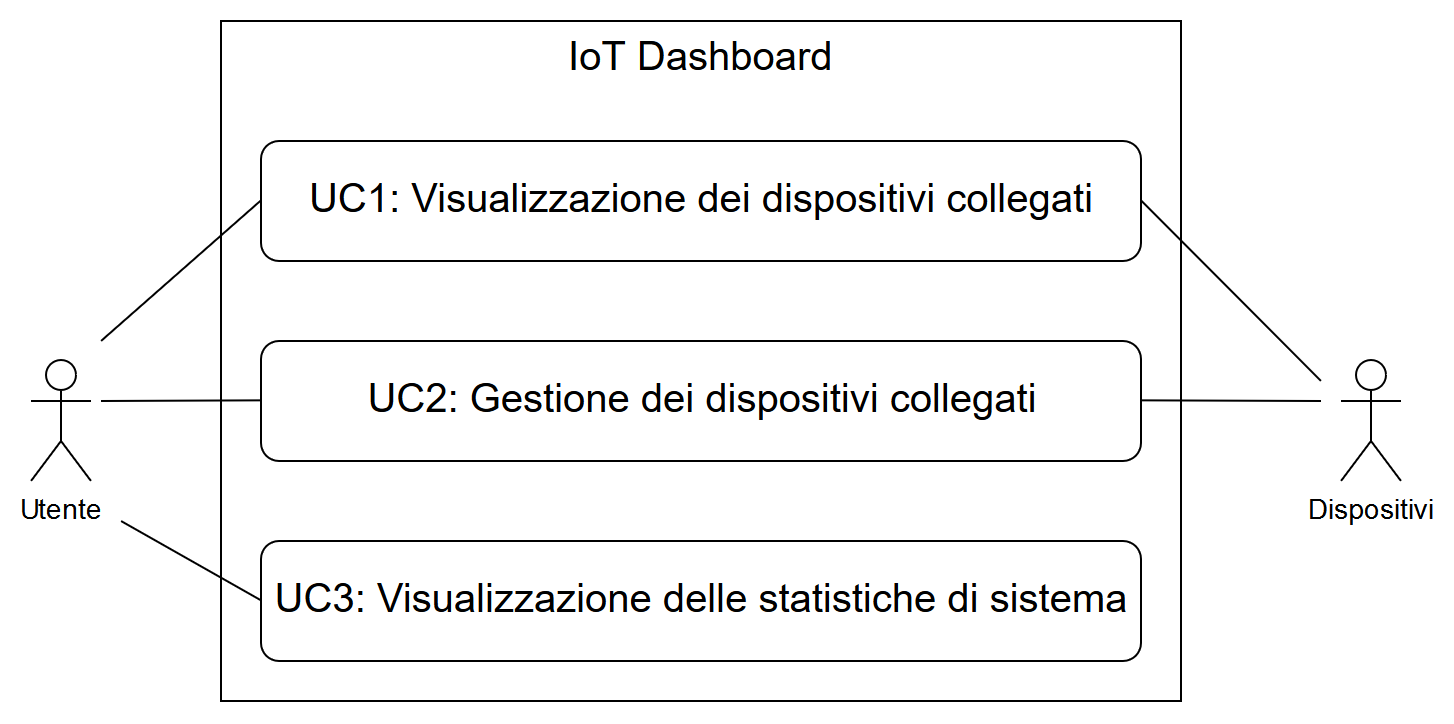
\includegraphics[width=0.9\columnwidth]{usecase/use_cases}
    \caption{Use Case - UC0: Scenario principale}
\end{figure}
% fine uc

% uc testuale
\begin{usecase}{1}{Visualizzazione dei dispositivi collegati}
\usecaseactors{Utente, Dispositivi}
\usecasepre{L'utente ha scelto di visualizzare tutti i dispositivi collegati}
\usecasedesc{L'utente interroga la \emph{dashboard} per conoscere lo stato dei dispositivi collegati}
\usecasepost{L'utente conosce lo stato di tutti i dispositivi collegati al sistema}
\label{uc:uc1}
\end{usecase}

% uc figura
\begin{figure}[!h]
    \centering
    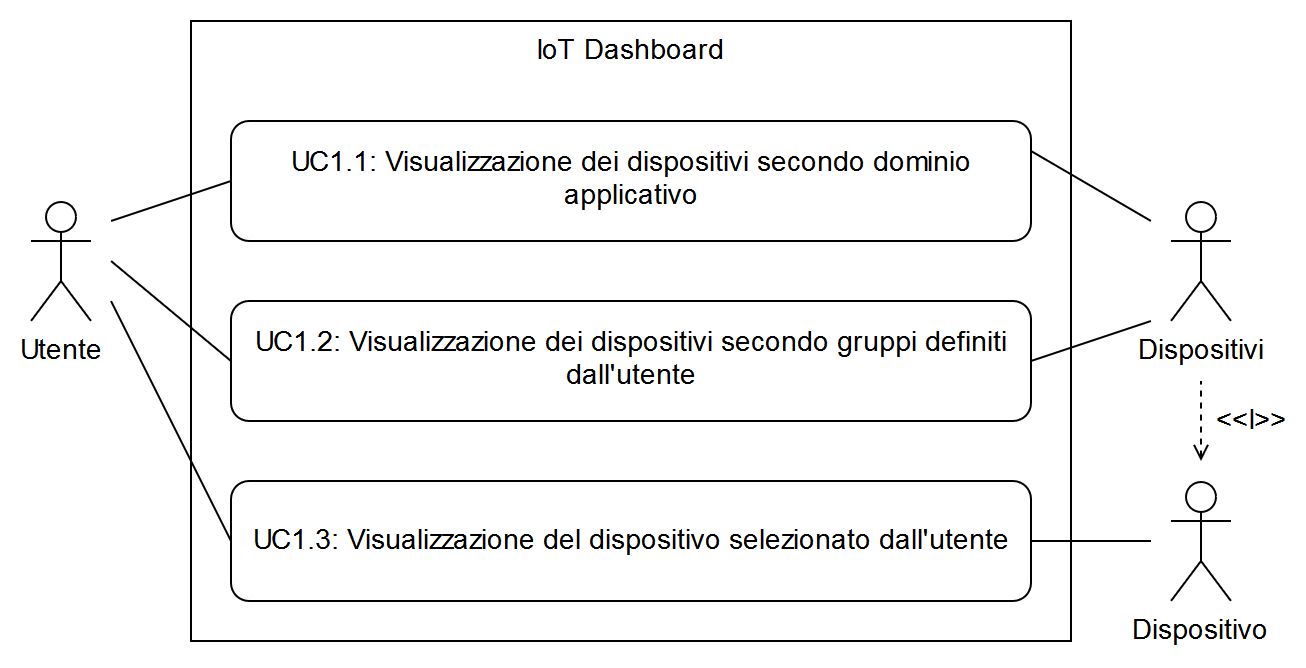
\includegraphics[width=0.9\columnwidth]{usecase/UC1}
    \caption{Use Case - UC1: Visualizzazione dei dispositivi collegati}
\end{figure}
% fine uc

% uc testuale
\begin{usecase}{1.1}{Visualizzazione dei dispositivi collegati secondo dominio applicativo}
\usecaseactors{Utente, Dispositivi}
\usecasepre{L'utente ha scelto di visualizzare tutti i dispositivi collegati}
\usecasedesc{L'utente interroga la dashboard per conoscere lo stato dei dispositivi collegati. In questa visualizzazione la dashboard mostra i dispositivi raggruppati secondo dominio applicativo (gruppo relativo alla termodinamica domestica, gruppo relativo alla illuminazione, ecc.)}
\usecasepost{L'utente conosce lo stato di tutti i dispositivi collegati al sistema secondo il dominio scelto}
\label{uc:uc1.1}
\end{usecase}
% fine uc

% uc testuale
\begin{usecase}{1.2}{Visualizzazione dei dispositivi collegati secondo gruppi definiti dall'utente}
\usecaseactors{Utente, Dispositivi}
\usecasepre{L'utente ha scelto di visualizzare tutti i dispositivi collegati}
\usecasedesc{L'utente interroga la dashboard per conoscere lo stato dei dispositivi collegati. In questa visualizzazione la dashboard mostra i dispositivi raggruppati secondo le preferenze dell'utente}
\usecasepost{L'utente conosce lo stato di tutti i dispositivi collegati al sistema presenti nel gruppo definito}
\label{uc:uc1.2}
\end{usecase}
% fine uc

% uc testuale
\begin{usecase}{1.3}{Visualizzazione del dispositivo selezionato dall'utente}
\usecaseactors{Utente, Dispositivi}
\usecasepre{L'utente ha scelto di visualizzare le informazioni di uno dei dispositivi collegati}
\usecasedesc{L'utente interroga la dashboard per conoscere lo stato del dispositivo selezionato. In questa visualizzazione la dashboard mostra le informazioni provenienti dal dispositivo}
\usecasepost{L'utente può visualizzare le informazioni specifiche del dispositivo}
\label{uc:uc1.3}
\end{usecase}
% fine uc

% uc testuale
\begin{usecase}{1.3.1}{Visualizzazione delle informazioni provenienti dal dispositivo}
\usecaseactors{Utente, Dispositivi}
\usecasepre{L'utente ha scelto di visualizzare le informazioni di uno dei dispositivi collegati}
\usecasedesc{La dashboard mostra all'utente le informazioni provenienti dal dispositivo}
\usecasepost{L'utente può visualizzare le informazioni specifiche del dispositivo}
\label{uc:uc1.3.1}
\end{usecase}
% fine uc

% uc testuale
\begin{usecase}{1.3.1.1}{Visualizzazione nome del dispositivo}
\usecaseactors{Utente, Dispositivi}
\usecasepre{L'utente ha scelto di visualizzare le informazioni di uno dei dispositivi collegati}
\usecasedesc{La dashboard mostra all'utente il nome \emph{user-friendly} dato dal produttore al dispositivo}
\usecasepost{L'utente conosce il nome dato dal produttore al dispositivo}
\label{uc:uc1.3.1.1}
\end{usecase}
% fine uc

% uc testuale
\begin{usecase}{1.3.1.2}{Visualizzazione categoria del dispositivo}
\usecaseactors{Utente, Dispositivi}
\usecasepre{L'utente ha scelto di visualizzare le informazioni di uno dei dispositivi collegati}
\usecasedesc{La dashboard mostra all'utente il dominio applicativo del dispositivo (illuminazione, ecc.)}
\usecasepost{L'utente conosce il dominio applicativo del dispositivo selezionato}
\label{uc:uc1.3.1.2}
\end{usecase}
% fine uc

% uc testuale
\begin{usecase}{1.3.1.3}{Visualizzazione dati provenienti dal dispositivo}
\usecaseactors{Utente, Dispositivi}
\usecasepre{L'utente ha scelto di visualizzare le informazioni di uno dei dispositivi collegati}
\usecasedesc{La dashboard mostra all'utente i dati raccolti dal sistema inviati dal dispositivo selezionato}
\usecasepost{L'utente conosce le misurazioni raccolte dal sistema per il dispositivo selezionato}
\label{uc:uc1.3.1.3}
\end{usecase}
% fine uc

% uc testuale
\begin{usecase}{1.3.2}{Visualizzazione delle specifiche tecniche del dispositivo}
\usecaseactors{Utente, Dispositivi}
\usecasepre{L'utente ha scelto di visualizzare le informazioni di uno dei dispositivi collegati}
\usecasedesc{La dashboard mostra all'utente le specifiche tecniche del dispositivo, quali produttore, modello, ecc.}
\usecasepost{L'utente conosce le specifiche tecniche del dispositivo selezionato}
\label{uc:uc1.3.2}
\end{usecase}
% fine uc

% uc testuale
\begin{usecase}{1.3.2.1}{Visualizzazione produttore del dispositivo}
\usecaseactors{Utente, Dispositivi}
\usecasepre{L'utente ha scelto di visualizzare le specifiche tecniche di uno dei dispositivi collegati}
\usecasedesc{La dashboard mostra all'utente il nome del produttore del dispositvo}
\usecasepost{L'utente conosce il nome del produttore del dispositivo selezionato}
\label{uc:uc1.3.2.1}
\end{usecase}
% fine uc

% uc testuale
\begin{usecase}{1.3.2.2}{Visualizzazione modello del dispositivo}
\usecaseactors{Utente, Dispositivi}
\usecasepre{L'utente ha scelto di visualizzare le specifiche tecniche di uno dei dispositivi collegati}
\usecasedesc{La dashboard mostra all'utente il nome commerciale scelto dal produttore per il dispositivo}
\usecasepost{L'utente conosce il nome commerciale del dispositivo selezionato}
\label{uc:uc1.3.2.2}
\end{usecase}
% fine uc

% uc testuale
\begin{usecase}{1.3.2.3}{Visualizzazione revisione del dispositivo}
\usecaseactors{Utente, Dispositivi}
\usecasepre{L'utente ha scelto di visualizzare le specifiche tecniche di uno dei dispositivi collegati}
\usecasedesc{La dashboard mostra all'utente un identificativo di versione del dispositivo (anno o  numero di versione)}
\usecasepost{L'utente conosce la revisione del dispositivo selezionato}
\label{uc:uc1.3.2.3}
\end{usecase}
% fine uc

% uc testuale
\begin{usecase}{1.3.3}{Visualizzazione delle operazioni disponibili per il dispositivo}
\usecaseactors{Utente, Dispositivi}
\usecasepre{L'utente ha scelto di visualizzare informazioni di uno dei dispositivi collegati}
\usecasedesc{La dashboard mostra all'utente le funzionalità offerte dal dispositivo}
\usecasepost{L'utente conosce la lista delle funzionalità offerte dal dispositivo selezionato}
\label{uc:uc1.3.3}
\end{usecase}
% fine uc

% uc testuale
\begin{usecase}{1.3.4}{Collegamento all'interfaccia proprietaria del dispositivo}
\usecaseactors{Utente, Dispositivi, Interfaccia proprietaria}
\usecasepre{L'utente ha scelto di visualizzare le informazioni di uno dei dispositivi collegati}
\usecasedesc{La dashboard mostra all'utente il collegamento all'interfaccia proprietaria del dispositivo}
\usecasepost{L'utentepuò seguire il collegamento per visualizzare l'interfaccia proprietaria del dispositivo selezionato}
\label{uc:uc1.3.4}
\end{usecase}
% fine uc

% uc testuale
\begin{usecase}{2}{Gestione dei dispositivi collegati}
\usecaseactors{Utente, Dispositivi}
\usecasepre{L'utente ha scelto di gestire i dispositivi collegati al sistema}
\usecasedesc{L'utente accede alla \emph{dashboard} per gestire i dispositivi collegati al sistema}
\usecasepost{L'utente può accedere alle funzionalità di gestione offerte dalla \emph{dashboard}}
\label{uc:uc2}
\end{usecase}
% fine uc

% uc testuale
\begin{usecase}{2.1}{Visualizzazione dei dispositivi collegati}
\usecaseactors{Utente, Dispositivi}
\usecasepre{L'utente ha scelto di gestire i dispositivi collegati al sistema}
\usecasedesc{La dashboard presenta all'utente la lista di dispositivi collegati al sistema per permettere all'utente di selezionare quale dispositivo gestire}
\usecasepost{L'utente può accedere alle funzionalità di gestione offerte dalla \emph{dashboard} per i dispositivi visualizzati}
\label{uc:uc2.1}
\end{usecase}
% fine uc

% uc testuale
\begin{usecase}{2.2}{Creazione di un gruppo di dispositivi personalizzato dall'utente}
\usecaseactors{Utente, Dispositivi}
\usecasepre{L'utente ha scelto di gestire i dispositivi collegati al sistema}
\usecasedesc{La dashboard permette all'utente di creare un gruppo personalizzato di dispositivi, facilitando la visualizzazione dei dispositivi nella pagina principale della \emph{dashboard}}
\usecasepost{L'utente ha creato un gruppo personalizzato con le proprietà richieste (nome e dispositivi)}
\label{uc:uc2.2}
\end{usecase}
% fine uc

% uc testuale
\begin{usecase}{2.2.1}{Inserimento nome del gruppo}
\usecaseactors{Utente}
\usecasepre{L'utente ha scelto di creare un gruppo personalizzato}
\usecasedesc{L'utente fornisce al sistema il nome del gruppo da creare}
\usecasepost{L'utente può proseguire nella creazione del gruppo personalizzato}
\label{uc:uc2.2.1}
\end{usecase}
% fine uc

% uc testuale
\begin{usecase}{2.2.2}{Scelta dei dispositivi da inserire nel gruppo}
\usecaseactors{Utente, Dispositivi}
\usecasepre{L'utente ha scelto di creare un gruppo personalizzato}
\usecasedesc{L'utente può selezionare i dispositivi che vuole raggruppare}
\usecasepost{L'utente ha creato un gruppo personalizzato con le proprietà specificate (nome e dispositivi)}
\label{uc:uc2.2.2}
\end{usecase}
% fine uc

% uc testuale
\begin{usecase}{2.3}{Modifica di un gruppo di dispositivi personalizzato}
\usecaseactors{Utente, Dispositivi}
\usecasepre{L'utente ha scelto di gestire i dispositivi collegati al sistema}
\usecasedesc{La dashboard permette all'utente di modificare un gruppo personalizzato esistente per rinominare il gruppo e aggiungere o togliere uno o più dispositivi da un gruppo}
\usecasepost{L'utente ha modificato il gruppo personalizzato esistente}
\label{uc:uc2.3}
\end{usecase}
% fine uc

% uc testuale
\begin{usecase}{2.3.1}{Modifica nome del gruppo}
\usecaseactors{Utente}
\usecasepre{L'utente ha scelto di modificare un gruppo personalizzato esistente}
\usecasedesc{La dashboard mostra all'utente il nome corrente del gruppo, permettendone la modifica}
\usecasepost{L'utente ha modificato il nome del gruppo personalizzato esistente}
\label{uc:uc2.3.1}
\end{usecase}
% fine uc

% uc testuale
\begin{usecase}{2.3.2}{Aggiunta di nuovi dispositivi al gruppo}
\usecaseactors{Utente, Dispositivi}
\usecasepre{L'utente ha scelto di modificare un gruppo personalizzato esistente}
\usecasedesc{La dashboard permette all'utente di scegliere quali dispositivi non presenti nel gruppo aggiungere}
\usecasepost{L'utente ha aggiunto i dispositivi selezionati al gruppo personalizzato esistente}
\label{uc:uc2.3.2}
\end{usecase}
% fine uc

% uc testuale
\begin{usecase}{2.3.3}{Rimozione di dispositivi esistenti dal gruppo}
\usecaseactors{Utente, Dispositivi}
\usecasepre{L'utente ha scelto di modificare un gruppo personalizzato esistente}
\usecasedesc{La dashboard permette all'utente di scegliere quali dispositivi presenti nel gruppo da rimuovere}
\usecasepost{L'utente ha rimosso i dispositivi selezionati al gruppo personalizzato esistente}
\label{uc:uc2.3.3}
\end{usecase}
% fine uc

% uc testuale
\begin{usecase}{2.4}{Rimozione di un gruppo di dispositivi personalizzato}
\usecaseactors{Utente}
\usecasepre{L'utente ha scelto di modificare un gruppo personalizzato esistente}
\usecasedesc{La dashboard permette all'utente di rimuovere un gruppo personalizzato esistente}
\usecasepost{L'utente ha rimosso il gruppo personalizzato esistente selezionato}
\label{uc:uc2.4}
\end{usecase}
% fine uc

% uc testuale
\begin{usecase}{2.5}{Visualizzazione delle operazioni disponibili per il dispositivo selezionato dall'utente}
\usecaseactors{Utente, Dispositivo}
\usecasepre{L'utente ha scelto di modificare un gruppo personalizzato esistente}
\usecasedesc{La dashboard permette all'utente di conoscere la lista delle operazioni disponibili per il dispositivo selezionato (ad esempio: accensione e spegnimento per una sorgente di illuminazione)}
\usecasepost{L'utente conosce la lista delle operazioni disponibili per il dispositivo selezionato}
\label{uc:uc2.5}
\end{usecase}
% fine uc

% uc testuale
\begin{usecase}{3}{Visualizzazione delle statistiche di sistema}
\usecaseactors{Utente}
\usecasepre{L'utente ha scelto di visualizzare lo stato del sistema}
\usecasedesc{L'utente interroga la dashboard per visualizzare le statistiche di sistema per conoscerne lo stato di salute e diagnosticare eventuali malfunzionamenti}
\usecasepost{L'utente conosce lo stato del sistema}
\label{uc:uc3}
\end{usecase}
% fine uc

% ## Requisiti
Presento di seguito i requisiti emersi durante l’analisi dei casi d’uso.
Per permetterne una consultazione agevole, ho deciso di inserire i requisiti in una tabella dei requisiti ~\ref{tab:requisiti}.
Nella tabella ~\ref{tab:requisiti}, presento i requisiti indicando:
\begin{itemize}
	\item Identificativo (secondo le regole indicate successivamente);
	\item Categoria di appartenenza fra:
	\begin{itemize}
		\item Obbligatorio, per i requisiti irrinunciabili;
		\item Desiderabile, per i requisiti non strettamente necessari ma che offrono un
    valore aggiunto riconoscibile;
		\item Opzionale, per i requisiti relativamente utili o contrattabili in seguito.
	\end{itemize}
	\item Descrizione esaustiva del requisito;
\end{itemize}

% ### Catalogazione requisiti
I requisiti sono identificati come segue:

\begin{figure}
  \centering
  \[ R[Categoria][Tipo][numero] \]
  \begin{tabular}{@{}>{$}l<{$}l@{}}
    R & specifica che si tratta di un requisito;\\
    Categoria & indica se si tratta di un requisito:
		\begin{itemize}
			\item Obbligatorio: `M` (\emph{mandatory});
			\item Desiderabile: `A` (\emph{advisable});
			\item Opzionale: `O` (\emph{optional});
		\end{itemize}
    Tipo & indica la tipologia del requisito, che può essere:
		\begin{itemize}
			\item Di vincolo: `O` (\emph{obligation});
			\item Funzionale: `F` (\emph{functional});
			\item Di qualità: `Q` (\emph{quality});
		\end{itemize}
		Numero & è assoluto e rappresenta un riferimento univoco al requisito in questione.\\
  \end{tabular}
\end{figure}

% ### Tabella dei requisiti

% #### Tabella dei requisiti di vincolo

\begin{table}[H]
\caption{Tabella dei requisiti di vincolo}
\label{tab:requisiti-vincolo}
\begin{tabularx}{\linewidth}{|c|c|X|}
\hline
\textbf{Identificativo} & \textbf{Categoria} & \textbf{Descrizione} \\
\hline
RMO1 & Obbligatorio & Il sistema deve essere progettato secondo lo stile di progettazione a microservizi. \\
\hline
RAO2 & Desiderabile & Il sistema può essere implementato utilizzando il linguaggio JavaScript secondo lo standard EcmaScript 2017. \\
\hline
RAO3 & Desiderabile & Il sistema può essere implementato utilizzando il framework Node.js per il \emph{backend} e React per il \emph{frontend}. \\
\hline
RMO4 & Obbligatorio & Il sistema deve utilizzare il protocollo MQTT. \\
\hline
\end{tabularx}
\end{table}

% #### Tabella dei requisiti funzionali

\begin{table}[H]
\caption{Tabella dei requisiti funzionali}
\label{tab:requisiti-funzionali}
\begin{tabularx}{\linewidth}{|c|c|X|}
\hline
\textbf{Identificativo} & \textbf{Categoria} & \textbf{Descrizione} \\
\hline
RMF1 & Obbligatorio & L'utente deve poter visualizzare tutti i dispositivi collegati al sistema. \\
\hline
RMF2 & Obbligatorio & L'utente deve poter visualizzare i dispositivi collegati secondo dominio applicativo. \\
\hline
RAF3 & Desiderabile & L'utente può visualizzare i dispositivi collegati secondo gruppi personalizzati. \\
\hline
RMF4 & Obbligatorio & L'utente deve poter selezionare uno dei dispositivi collegati per visualizzarne le informazioni. \\
\hline
RAF5 & Desiderabile & L'utente può creare un gruppo di dispositivi personalizzato. \\
\hline
RAF6 & Desiderabile & L'utente può modificare uno dei gruppi personalizzati esistenti. \\
\hline
RAF7 & Desiderabile & L'utente può rimuovere uno dei gruppi di dispositivi personalizzati esistenti. \\
\hline
RMF8 & Obbligatorio & L'utente deve poter visualizzare le operazioni messe a disposizione dal dispositivo selezionato. \\
\hline
RMF9 & Obbligatorio & L'utente deve poter selezionare una delle operazioni disponibili. \\
\hline
RMF10 & Obbligatorio & L'utente deve poter visualizzare le statistiche di utilizzo del sistema sistema. \\
\hline
\end{tabularx}
\end{table}

% #### Tabella dei requisiti di qualità

\begin{table}[H]
\caption{Tabella dei requisiti di qualità}
\label{tab:requisiti-qualita}
\begin{tabularx}{\linewidth}{|c|c|X|}
\hline
\textbf{Identificativo} & \textbf{Categoria} & \textbf{Descrizione} \\
\hline
ROQ1 & Opzionale & Il sistema deve essere testato, raggiungendo i seguenti obiettivi:
\begin{itemize}
	\item \emph{statement coverage} > 80 \%
	\item \emph{branch coverage} > 90 \%
\end{itemize}
\hline
\end{tabularx}
\end{table}

\begin{table}[H]
\caption{Tabella di riepilogo dei requisiti}
\label{tab:requisiti-riepilogo}
\begin{tabularx}{\linewidth}{|c|c|X|}
\hline
\textbf{Tipo} & \textbf{Obbligatorio} & \textbf{Opzionale} & \textbf{Desiderabile} \\
\hline
Funzionale & 6 & 0 & 4 \\
\hline
Qualitativo & 0 & 1 & 0 \\
\hline
Di vincolo & 2 & 0 & 2 \\
\hline
Totale & 8 & 1 & 6 \\
\hline
\end{tabularx}
\end{table}

%**************************************************************
\section{Progettazione}

### Scopo del documento

Lo scopo di questo documento è quello di definire la progettazione dell'architettura ad alto livello del progetto di stage.
Il presente, tra le altre cose, tratta di:

-   tecnologie utilizzate;
-   architettura del sistema e dei relativi componenti software;
-   Design Pattern<sub>[1](#1)</sub> impiegati per la progettazione.

### Scopo del progetto

Lo stage prevede lo sviluppo e la realizzazione di una dashboard per la gestione di dispositivi interconnessi (IoT). L'idea alla base del sistema è quella di un centro di controllo attraverso cui l'utente del sistema gestisca i dispositivi smart presenti nella propria rete domestica.

## Architettura


L'architettura scelta per il sistema segue lo stile architetturale a microservizi con l'obiettivi di approfondire questo stile architetturale e implementarlo in uno scenario plausibile.
Lo stile architetturale a microservizi descrive un metodo di progettazione delle applicazioni come **insiemi di servizi eseguibili indipendentemente**, **che comunicano tra loro grazie a meccanismi di comunicazione leggeri**.

![Panoramica sull'architettura software](./images/arch-overview.png)

### Servizio: MQTT Broker

Il broker MQTT è il servizio resonsabile alla ricezione di tutti i messaggi, alla loro catalogazione e all'invio delle notifiche verso i client sottoscritti a ciascuna categoria.
Il broker memorizza lo stato di tutti i client a lui connessi, inclusi i messaggi non ancora inviati o il cui invio è fallito.

### Servizio: termometro _virtualizzato_

Questo servizio simula la presenza di un sensore che invii dati sulla temperatura dell'ambiente in cui si trova.

Esso pubblica periodicamente la temperatura rilevata secondo l'argomento `temperature` e secondo l'argomento `hw_info` i propri dati identificativi, quali produttore, modello, ecc.

Data la relativa importanza i dati vengono inviati con un QoS di livello 0 nella categoria `temperature`, mentre con QoS di livello 1 nella categoria `hw_info`.

Anche se nel diagramma è disegnato individualmente, è possibile che ve ne siano molteplici.

#### Servizio: termometro _virtualizzato_ - Panoramica delle classi

![Panoramica delle classi del servizio di simulazione di un  termometro](./images/virtual_temp_sensor_classes.png)

Classe                        | Funzionalità
------------------------------|-------------------------------------------------------------------------------------------------------------------------------------------------------------------------------------------------
`DeviceInfo`                  | Classe i cui oggetti rappresentano le informazioni del dispositivo, quali produttore, modello, revisione, ecc. Questi dati vengono pubblicati nel topic `hw_info`.
`ServiceManager`              | Classe responsabile dell'integrazione tra generazione dei dati di temperatura, gestione delle informazioni del dispositivo e invio delle informazioni tramite protocollo MQTT.
`MQTTClient`                  | Classe utile all'inizializzazione del client MQTT.
`TemperatureCurveFactory`     | Classe Factory astratta che espone la funzionalità di creazione della curva di temperatura, rappresentata dalla classe `TemperatureCurve`.
`SineTemperatureCurveFactory` | Implementazione della factory `TemperatureCurveFactory` per la creazione di oggetti `SineTemperatureCurve`.
`TemperatureCurve`            | Classe astratta che espone le funzionalità di inizializzazione della funzione, di aggiunta di rumore pseudocasuale nella funzione creata e di simulazione della temperatura data l'ora corrente.
`SineTemperatureCurve`        | Classe che implementa `TemperatureCurve` definendo una funzione di simulazione sinusoidale, in cui i parametri modificabili sono ampiezza, frequenza e fase.

### Servizio: temperatura

Questo servizio si occupa di raccogliere tutti i dati provenienti dai sensori di temperatura, memorizzandoli e mettendoli a disposizione in un formato strutturato per gli altri servizi del sistema.

Il servizio si sottoscrive alla categoria `temperature` e comunica con un QoS di livello 0, inoltre può pubblicare messaggi con la sottocategoria `temperature/active` per usufruire delle funzionalità aggiuntive presenti in dispositivi attivi legati alla temperatura.

#### Servizio: temperatura - Panoramica delle classi

![Panoramica delle classi del servizio legato al controllo temperatura](./images/temperature_service_classes.png)

Classe            | Funzionalità
------------------|--------------------------------------------------------------------------------------------------------------------------------------------------------------------------
`ServiceManager`  | Classe responsabile dell'integrazione tra ricezione dei dati di temperatura, gestione della persistenza dei dati ed esposizione di una interfaccia per gli altri servizi.
`MQTTClient`      | Classe utile all'inizializzazione del client MQTT.
`DBClient`        | Classe utile all'inizializzazione del client per il database del servizio.
`API`             | Classe che rappresenta le funzionalità esposte all'esterno dal servizio.
`TemperatureData` | Classe che rappresenta i dati ricevuti dai dispositivi attraverso il protocollo MQTT.

### Servizio: lampada _virtualizzata_

Questo servizio simula la presenza di un dispositivo _attivo_: una lampada in grado di comunicare il proprio assorbimento energetico e la sua durata stimata.
La lista delle operazioni disponibili è la seguente:

1.  accensione della lampada (QoS di livello 1);
2.  spegnimento della lampada (QoS di livello 1);
3.  richiesta assorbimento energetico (QoS di livello 0);
4.  richiesta tempo di vita stimato della lampada (QoS di livello 0).

L'argomento a cui la lampada si sottoscrive è `light/active`, in quanto capace di rispondere a richieste più complesse. Al primo collegamento il dispositivo invia i propri dati identificativi, pubblicandoli nella categoria `hw_info`.

#### Servizio: lampada _virtualizzata_ - Panoramica delle classi

![Panoramica delle classi del servizio di simulazione di una  lampada](./images/virtual_lamp_classes.png)

Classe           | Funzionalità
-----------------|-------------------------------------------------------------------------------------------------------------------------------------------------------------------
`DeviceInfo`     | Classe i cui oggetti rappresentano le informazioni del dispositivo, quali produttore, modello, revisione, ecc. Questi dati vengono pubblicati nel topic `hw_info`.
`ServiceManager` | Classe responsabile dell'integrazione tra stato della lampada e invio delle informazioni tramite protocollo MQTT.
`MQTTClient`     | Classe utile all'inizializzazione del client MQTT.
`Lamp`           | Classe che utilizza il Design Pattern Singleton per fornire lo stato della lampada (on/off).

### Servizio: illuminazione

Questo servizio si occupa di raccogliere e memorizzare tutti i dati pubblicati dai dispositivi nella categoria `light` e permette il controllo dei dispositivi sottoscritti alla categoria `light/active`.

Questo servizio utilizza sia QoS di livello 0 che di livello 1.

#### Servizio: illuminazione - Panoramica delle classi

![Panoramica delle classi del servizio legato all'illuminazione](./images/light_service_classes.png)

Classe                  | Funzionalità
------------------------|--------------------------------------------------------------------------------------------------------------------------------------------------------------------------------------------
`ServiceManager`        | Classe responsabile dell'integrazione tra ricezione dei dati dei dispositivi di illuminazione, gestione della persistenza dei dati ed esposizione di una interfaccia per gli altri servizi.
`MQTTClient`            | Classe utile all'inizializzazione del client MQTT.
`DBClient`              | Classe utile all'inizializzazione del client per il database del servizio.
`API`                   | Classe che rappresenta le funzionalità esposte all'esterno dal servizio. Include anche l'interfaccia di controllo dei dispositivi di illuminazione "_attivi_".
`LightData`             | Classe che rappresenta i dati ricevuti dai dispositivi attraverso il protocollo MQTT.
`RGBLightDataDecorator` | Classe che aggiunge informazioni relative alla temperatura colore della luce emessa dal dispositivo.
`LightController`       | Classe che permette di controllare i dispositivi collegati, preparando i pacchetti che la classe `API` può inviare ai dispositivi secondo l'interfaccia definita dal produttore.

### Servizio: informazioni dispositivo

Questo servizio si occupa di raccogliere e memorizzare tutti i dati pubblicati secondo l'argomento `hw_info`.

Il servizio utilizza esclusivamente un livello di QoS pari a 1 per aumentare l'affidabilità del sistema a fronte delle attività di identificazione dei dispositivi collegati.

#### Servizio: informazioni dispositivo - Panoramica delle classi

![Panoramica delle classi del servizio legato alle informazioni dei dispositivi](./images/devicesinfo_service_classes.png)

Classe                            | Funzionalità
----------------------------------|-----------------------------------------------------------------------------------------------------------------------------------------------------------------------------------
`ServiceManager`                  | Classe responsabile dell'integrazione tra ricezione dei dati dei dispositivi, gestione della persistenza dei dati ed esposizione di una interfaccia per gli altri servizi.
`MQTTClient`                      | Classe utile all'inizializzazione del client MQTT.
`DBClient`                        | Classe utile all'inizializzazione del client per il database del servizio.
`API`                             | Classe che rappresenta le funzionalità esposte all'esterno dal servizio, permettendo di richiedere i dati dei dispositivi e fornire la specifica dei dati inviati dai dispositivi.
`DeviceInfo`                      | Classe che rappresenta le informazioni di base ricevute dai dispositivi attraverso il protocollo MQTT.
`ActiveDeviceOperations`          | Classe che contiene la lista delle operazioni messe a disposizione dai dispositivi "_attivi_".
`ActiveDeviceOperationDescriptor` | Classe che contiene le specifiche della funzionalità messa a disposizione dal dispositivo.

### Servizio: preferenze utente

Questo servizio si occupa di salvare le preferenze utente, quali ad esempio gruppi personalizzati, unità di misura preferite, ecc.

Il servizio non utilizza il protocollo MQTT, bensì viene utilizzato solamente dal servizio **API**.

#### Servizio: preferenze utente - Panoramica delle classi

![Panoramica delle classi del servizio di trattamento delle preferenze utente](./images/userpreference_service_classes.png)

Classe                            | Funzionalità
----------------------------------|-----------------------------------------------------------------------------------------------------------------------------------------------------------------------------------
`ServiceManager`                  | Classe responsabile della gestione della persistenza delle preferenze utente e dell'esposizione di una interfaccia per gli altri servizi.
`DBClient`                        | Classe utile all'inizializzazione del client per il database del servizio.
`API`                             | Classe che rappresenta le funzionalità esposte all'esterno dal servizio, permettendo di richiedere e modificare le preferenze dell'utente.
`UserData`                      | Classe che rappresenta le informazioni di base dell'utente (nome, cognome, ecc.).
`SystemUnitDefinition`          | Classe che contiene la lista delle unità di misura scelte dall'utente per ogni metrica.
`UnitsConverter` | Classe che espone la funzionalità di conversione unità di misura.

### Servizio: API

Questo servizio svolge un ruolo da intermediario tra il servizio che fornisce l'applicazione web e il broker MQTT.

Esso interroga i servizi **illuminazione**, **temperatura** e **informazioni dispositivo**  definiti dal sistema per fornire una interfaccia unificata ai dati, sia in maniera sincrona sia in maniera asincrona.

L'interfaccia sincrona consiste in un'interfaccia che risponde ai metodi HTTP, mentre l'interfaccia asincrona richiede l'istituzione di una connessione che utilizzi i WebSocket.

#### Servizio: API - Panoramica delle classi

![Panoramica delle classi del servizio di gateway delle API](./images/api_service_classes.png)

Classe             | Funzionalità
-------------------|-----------------------------------------------------------------------------------------------------------------------------------------
`ServiceManager`   | Classe responsabile dell'integrazione tra istanza del server e interfaccia ai dati esposta.
`Server`           | Classe responsabile del ciclo di vita del server Node.js.
`Route`            | Interfaccia che mette espone i metodi e le proprietà necessarie alla creazione degli endpoint dati.
`UserRoute`        | Implementazione di `Route` che rappresenta gli endpoint per la gestione dell'utente.
`DevicesRoute`     | Implementazione di `Route` che rappresenta gli endpoint messi a disposizione per la ricerca e identificazione dei dispositivi collegati.
`TemperatureRoute` | Implementazione di `Route` che espone le funzionalità di gestione della temperatura.
`LightRoute`       | Implementazione di `Route` che espone le funzionalità di gestione dell'illuminazione.

### Servizio: web app

Questo servizio comprende l'applicazione web per la consultazione del sistema per mezzo dei browser.

Richiede i dati direttamente al servizio **API**, in particolare presentando i dati ottenuti in tempo reale con l'interfaccia asincrona del servizio **API**.

#### Servizio: web app - Panoramica delle classi

![Panoramica delle classi del servizio web app](./images/web_service_classes.png)

Classe               | Funzionalità
---------------------|-------------------------------------------------------------------------------------------------------------------------------------------------------------------------------------------------
`ServiceManager`     | Classe responsabile dell'integrazione tra istanza del server, pagine esposte e interfaccia di richeista dati.
`DataFetcher`  | Modulo che si occupa di effettuare le richieste al servizio **API** secondo le definizioni specificate in ingresso.
`Server`             | Classe responsabile del ciclo di vita del server Node.js. Effettua le richieste definite dalle `UIRoute` per ricevere i dati, utilizzando `DataFetcher`.
`UIRoute`            | Interfaccia utilizzata per definire le richieste da effettuare per ricevere le informazioni che popolano le pagine della rotta.
`UserUIRoute`        | Implementazione di `UIRoute` che definisce le richieste per ottenere o modificare le preferenze dell'utente e le pagine di visualizzazione e modifica delle preferenze utente.
`DevicesUIRoute`     | Implementazione di `UIRoute` che definisce le richieste per ottenere informazioni sui dispositivi collegati e le pagine di visualizzazione di questi.
`TemperatureUIRoute` | Implementazione di `UIRoute` che definisce le richieste per ottenere dati legati alla temperatura, visualizzare ed eseguire operazioni con dispositivi attivi e ne permette la visualizzazione.
`LightUIRoute`       | Implementazione di `UIRoute` che definisce le richieste per ottenere dati legati all'illuminazione, visualizzare ed eseguire operazioni con dispositivi attivi e ne permette la visualizzazione.
`UIPage`             | Implementazione di un componente React (`React.Component`) che rappresenta una pagina. La pagina visualizzata può contenere più figli anch'essi componenti React.
`React.Component`    | Classe che rappresenta un componente grafico nel framework React.


## Design Pattern

I Design Pattern descrivono la metodologia con cui affrontare problemi ricorrenti, fornendo soluzioni standard condivise.
La conoscenza dei Design Pattern favorisce la progettazione, il riuso e la manutenibilità del codice prodotto.
I principali Design Pattern vengono suddivisi in quattro categorie:
-   Architetturali: affrontano il problema di progettazione di un sistema software fornendo uno schema di partenza su cui basare l’architettura;
-   Creazionali: affrontano il problema di astrarre il sistema rendendolo indipendente dall’implementazione concreta delle sue componenti;
-   Strutturali: affrontano il problema riguardante la composizione delle classi e degli oggetti, sfruttando l’ereditarietà e l’aggregazione;
-   Comportamentali: affrontano il problema dell’interazione tra le componenti, definendo la funzione degli oggetti e il modo in cui interagiscono gli uni con gli altri.

### Design Pattern Comportamentali

#### Mediator

Il design pattern **Mediator** ha l'intento di disaccoppiare entità del sistema che devono comunicare fra loro. Il pattern infatti fa in modo che queste entità non si referenzino reciprocamente, agendo da "mediatore" fra le parti.

##### Utilizzo

Questo pattern è utilizzato in tutti i servizi sottoforma della classe `ServiceManager` per aumentare il disaccoppiamento tra classi che trattano la persistenza, l'esecuzione dei servizi, la comunicazione, ecc.

### Design Pattern Creazionali

#### Abstract Factory

L'**Abstract Factory** fornisce un'interfaccia per creare famiglie di oggetti connessi o dipendenti tra loro, in modo che non ci sia necessità da parte dei client di specificare quale classe istanziare, permettendo che un sistema sia indipendente dall'implementazione degli oggetti concreti e che il client, attraverso l'interfaccia, utilizzi diverse famiglie di prodotti.

##### Utilizzo

Questo pattern è utilizzato nel servizio [Servizio: termometro _virtualizzato_](#user-content-servizio-termometro-virtualizzato) per permettere la creazione di funzioni di generazione della temperatura.

![Utilizzo del pattern Abstract Factory](./images/abstract_factory.png)

#### Singleton

Il **Singleton** ha lo scopo di garantire che di una determinata classe venga creata una e una sola istanza, fornendo un unico punto di accesso globale a tale istanza.

##### Utilizzo

Questo pattern è utilizzato nel servizio [Servizio: lampada _virtualizzata_](#user-content-servizio-lampada-virtualizzata) per obbligare il servizio a simulare una singola lampada, favorendo così l'esecuzione di numerosi container del servizio per simulare un intero sistema d'illuminazione.

![Utilizzo del pattern Singleton](./images/singleton.png)

### Design Pattern Strutturali

#### Decorator

Il design pattern **Decorator** consente di aggiungere nuove funzionalità ad oggetti già esistenti, senza utilizzare l'ereditarietà tra classi.

##### Utilizzo

Questo pattern è utilizzato nel servizio [Servizio: illuminazione](#user-content-servizio-illuminazione) per permettere al servizio di aggiungere dinamicamente le funzionalità di cambiamento colore ad una sorgente luminosa normale.

![Utilizzo del pattern Decorator](./images/decorator.png)

#### Composite

Il design pattern **Composite** organizza gli oggetti in una struttura ad albero, nella quale i nodi sono delle entità composte e le foglie sono oggetti semplici.

##### Utilizzo

Questo pattern è utilizzato nel servizio [Servizio: web app](#user-content-servizio-web-app) per permettere la composizione di più componenti React per costruire interfacce complesse.

![Utilizzo del pattern Composite](./images/composite.png)

#### Module

Il pattern **Module** è uno dei pattern specifici del linguaggio JavaScript: il suo scopo è quello di rendere disponibile all’interno degli oggetti l’encapsulation, mantenendo privati e non accessibili dall’esterno campi dati e funzioni utilizzate internamente.


%**************************************************************
\section{Documentazione}

Come è stata prodotta la documentazione? A chi è rivolta? Come è documentato il codice?

%**************************************************************
\section{Test}

Come sono stati svolti i test? Coverage?


%**************************************************************
\section{Validazione dei Requisiti}

Quali requisiti sono stati rispettati e quali invece sono stati abbandonati.
